\documentclass[a4paper]{article}
\usepackage[UTF8]{ctex}
\usepackage{geometry}
\usepackage{graphicx}
\usepackage{url}
\usepackage{multirow}
\usepackage{array}
\usepackage{booktabs}
\usepackage{url}
\usepackage{enumitem}
\usepackage{graphicx}
\usepackage{float}
\usepackage{amssymb}
\usepackage{amsmath}
\usepackage{subfig}
\usepackage{longtable}
\usepackage{pifont}

\allowdisplaybreaks


\geometry{a4paper, scale=0.78}

% \begin{figure}[H]
%     \centering
%     \includegraphics[width=.55\textwidth]{E.png}
%     \caption{矩阵与列向量的乘法}
%     \label{fig:my_label_1}
% \end{figure}

% \left\{
% \begin{array}{ll}
%       x+2x+z=2 & \\
%       3x+8y+z=12 & \\
%       4y+z=2
% \end{array}
% \right.

% \begin{enumerate}[itemindent = 1em, itemsep = 0.4pt, parsep=0.5pt, topsep = 0.5pt]

% \end{enumerate}

\title{Linear Classification 06 Naive Bayes}
\author{Chen Gong}
\date{04 November 2019}

\begin{document}
\maketitle

本节主要是介绍一下Naive Bayes Classification,也就是朴素贝叶斯分类。朴素贝叶斯分类器的核心思想也就是,条件独立性假设。这是一种最简单的概率图模型,也就是一种有向图模型。

\section{条件独立性假设}
条件独立性假设用简单的图来进行表述,可以表示为如下图所示的形式:
\begin{figure}[H]
    \centering
    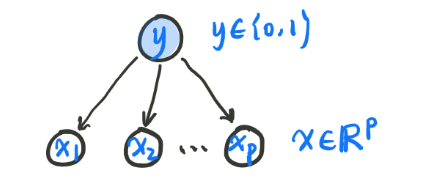
\includegraphics[width=.55\textwidth]{微信图片_20191104091918.png}
    \caption{条件独立性假设}
    \label{fig:my_label_1}
\end{figure}

我们可以将其定义为$x_i\perp x_j|y\ (i \neq j)$。根据贝叶斯公式可以得:
\begin{equation}
    p(y|x)=\frac{p(x|y)p(y)}{p(x)}=\frac{p(x,y)}{p(x)}\propto p(x,y)
\end{equation}

而做条件独立性假设的最终目的,是为了简化运算。因为对于一个数据序列$x=(x_1,x_2,\cdots,x_p)$。如果$x_i$和$x_j$之间有关系的话,这个计算难度可能会变得很难,所以就假设各个变量之间是相互独立的。而且,马尔可夫决策链也就是这样类似的思想。

\section{Naive Bayes Classification}
朴素贝叶斯算法的优化目的即为:
\begin{equation}
    \begin{split}
        \hat{y} = & \arg\max_{y\in \{0,1\}}p(y|x) \\
        = & \arg\max_{y\in \{0,1\}}p(x|y)p(y) \\
    \end{split}
\end{equation}

其中,
\begin{equation}
    p(x|y) = \prod_{i=1}^Np(x_i|y)
\end{equation}

对于$p(y)$这个先验概率密度函数的确定,对于二分类问题,也就是$y\sim$Bernoulli Distribution,而对于多分类问题,先验概率为$y\sim$Categorial Distribution。而对于,$p(x|y) = \prod_{i=1}^Np(x_i|y)$。如果$x$是离散的,那么$x_i|y\sim$Categorial Distribution;如果$x$是连续的,那么$x_i|y\sim\mathcal{N}(\mu_y,\Sigma^2_y)$。对于每一类都有一个高斯分布。

而有关于$p(x|y)$用极大似然估计MLE,估计出来就行。因为分布的形式我们已经知道了,那么只要利用数据来进行学习,使用极大似然估计就可以得到想要的结果了。其实对于多分类的情况,Naive Bayes Classification和Guassian Discriminate Analysis很像的。


\end{document}
